% 2012 年陕西卷理科第 18 题：平面 π 内的直线 a，π 外的直线 b 及其投影 c。
% 来源 PDF：普通高考/2012/2012陕西理.pdf，第 2 页（印面 764）第 1 栏。
% 斜二测画平面 π 为平行四边形；b 从平面上方斜穿，c 为其在 π 上的投影。
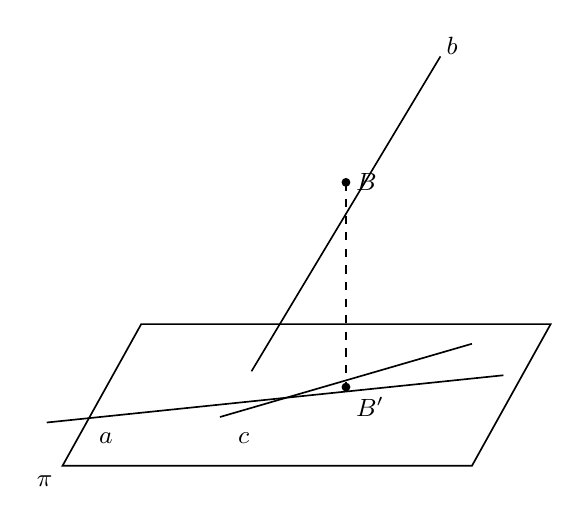
\begin{tikzpicture}[semithick, font=\small]
  % 平面 π
  \draw (0,0) -- (5.2,0) -- (6.2,1.8) -- (1.0,1.8) -- cycle;
  \node[below left] at (0,0) {$\pi$};
  % 直线 a（在平面内）
  \draw (-0.2,0.55) -- (5.6,1.15);
  \node[below] at (0.55,0.55) {$a$};
  % 投影 c（在平面内）
  \coordinate (B) at (3.6,3.6);
  \coordinate (Bp) at (3.6,1.0);
  \draw (2.0,0.62) -- (5.2,1.55);
  \node[below] at (2.3,0.55) {$c$};
  % 直线 b 及垂线 BB'
  \draw (2.4,1.2) -- (4.8,5.2);
  \node[above right] at (4.75,5.1) {$b$};
  \draw[dashed] (B) -- (Bp);
  \fill (Bp) circle (1.6pt);
  \node[below right] at (Bp) {$B'$};
  \fill (B) circle (1.6pt);
  \node[right] at (B) {$B$};
\end{tikzpicture}
